\subsection{Slave Jordfugt Design}
\label{ch:slave_jordfugt_design}

Slave Jordfugt er tilkoblet op til seks analoge jordfugtsensorer, og den har til opgave at indsamle data fra disse og kommunikere med PSoC Master på \IIC bussen.
Figur \ref{fig:stm_jordfugt} viser en state machine for SW på PSoC 4 i Slave Jordfugt. 
ADC'en i PSoC 4 står hele tiden og opdaterer seks registre, uanset hvad PSoC'en ellers laver. 
Koden er derfor designet sådan, at når der modtages besked om at læse på en given sensor, opdateres en variabel (\texttt{index}), hvorefter data fra den pågældende sensor lægges i read bufferen.

\begin{figure}[h]
\centering 
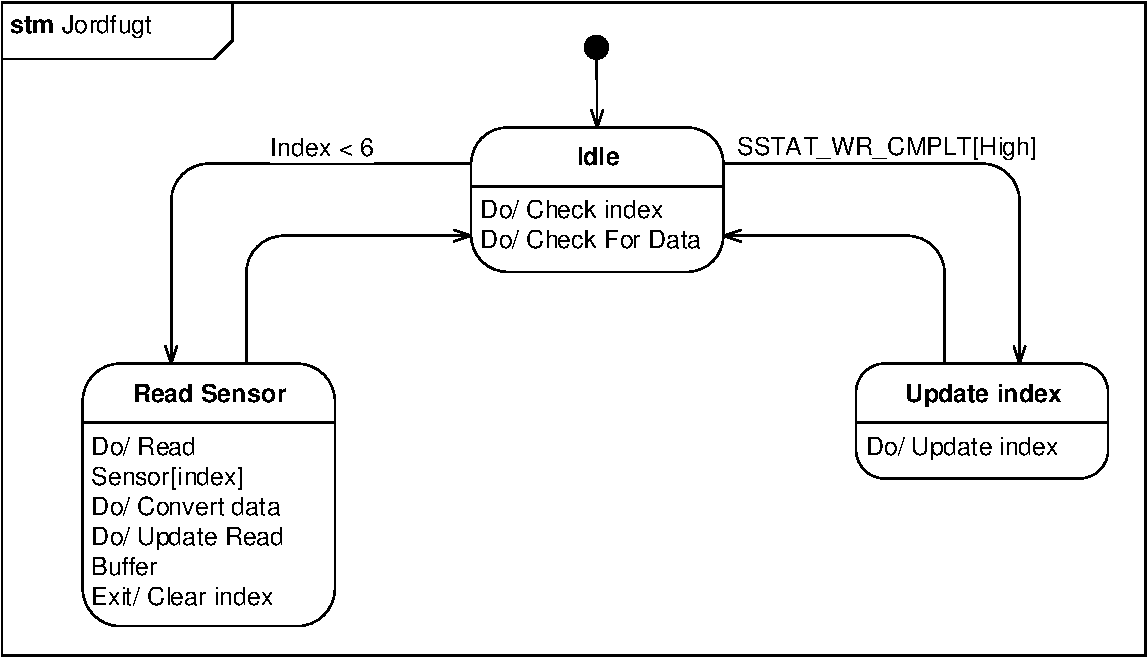
\includegraphics[width={\textwidth}, trim=0 0 0 0, clip=true] {../fig/stm_jordfugt.pdf}
\caption{State Machine for SW på PSoC 4 i blokken Jordfugt}
\label{fig:stm_jordfugt}
\end{figure}

De anvendte sensorer er indkøbt, men der foreligger ikke datablad eller lignende.
Under MSE øvelse 6, blev der lavet en undersøgelse af sensorernes virkemåde, herunder primært støjmåling \cite{lib:MSE_06}.

\clearpage